\documentclass[11pt]{article}

\usepackage{amsmath, amssymb, amsthm} % ams packages %amsfonts is loaded by amssymb
\usepackage[all,warning]{onlyamsmath}
\usepackage{graphics, graphicx} % graphics packages


\usepackage[margin=1in]{geometry} % more reasonable margins
\usepackage{booktabs} % prettier tables
\usepackage{units} % prettier fractions (?)

% Small sections of multiple columns
\usepackage{multicol}

\usepackage{bm}
\usepackage{url}

\usepackage{natbib}

\usepackage{tikz} % make graphics in latex
\usetikzlibrary{shapes,decorations}
\usetikzlibrary{arrows}
\usepackage{pgfplots} % to make plots in latex
\pgfplotsset{compat=newest} % compatibility issue
\usepackage{enumitem, comment}

% formatting
\usepackage{fancyhdr} % for changing headers and footers
\usepackage{url} % url 
\usepackage[normalem]{ulem}
\usepackage{color} % colored text + names %deprecated?



% hyperlink in the document
\usepackage{hyperref} % must be the last package loaded

\usepackage{comment}

\usepackage{parskip}

% notations
\newcommand{\one}{\ensuremath{\mathbf{1}}}
\newcommand{\zero}{\ensuremath{\mathbf{0}}}
\newcommand{\prob}{\ensuremath{\mathbf{P}}}
\newcommand{\expec}{\ensuremath{\mathbf{E}}}
\newcommand{\ind}{\ensuremath{\mathbf{I}}}
\newcommand{\reals}{\ensuremath{\mathbb{R}}}
\newcommand{\naturals}{\ensuremath{\mathbb{N}}}
\newcommand{\defeq}{\ensuremath{\triangleq}}
\newcommand{\sP}{\ensuremath{\mathsf{P}}}
\newcommand{\sQ}{\ensuremath{\mathsf{Q}}}
\newcommand{\sE}{\ensuremath{\mathsf{E}}}

\newcommand{\mbf}[1]{{\boldsymbol{\mathbf{#1}}}}
\renewcommand{\bm}{\mbf}


% environments
\newtheorem{theorem}{Theorem}
\newtheorem{proposition}{Proposition}
\newtheorem{corollary}{Corollary}
\newtheorem{lemma}{Lemma}
\newtheorem{remark}{Remark}
\newtheorem{definition}{Definition}
\newtheorem{assumption}{Assumption}



\title{\vspace{-20mm} Bayesian Machine Learning}
\date{}
\author{
\textbf{Homework 3}  \\ \textbf{Due: Tuesday, October 20, 11:55 pm}}
\begin{document}
\maketitle

\

\textbf{Model Comparison, Occam's Razor, and the Laplace Approximation} \\
(49 marks) \\ \\

The \emph{evidence} $p(\mathcal{D}|\mathcal{M})$, also known as the \emph{marginal likelihood}, is the probability that if we were to randomly sample parameters $\bm{\theta}$ from $\mathcal{M}$ that we would create dataset $\mathcal{D}$: 
\begin{align}
p(\mathcal{D} | \mathcal{M}) = \int p(\mathcal{D} | \mathcal{M}, \bm{\theta}) p(\bm{\theta} | \mathcal{M}) d\bm{\theta}
\label{eqn: evidence}
\end{align}
Simple models $\mathcal{M}$ can only generate a small number
of datasets, but because the marginal likelihood must normalise, it will generate these datasets with
high probability. Complex models can generate a wide range of datasets, but each with typically low
probability. For a given dataset, the marginal likelihood will favour a model of more appropriate
complexity, as illustrated in Figure~\ref{fig: occam}.


\begin{enumerate}
\item (12 marks): Consider the Bayesian linear regression model, 
\begin{align}
y &= \bm{w}^{\top} \bm{\phi}(\bm{x},\bm{z}) + \epsilon(\bm{x})   \\
\epsilon(\bm{x}) &\sim \mathcal{N}(0,\sigma^2) \\
p(\bm{w}) &= \mathcal{N}(0,\alpha^2 I) 
\end{align}
where the data $\mathcal{D}$ consist of $N$ input-output pairs, $\{\bm{x}_i, y_i\}_{i=1}^{N}$, $\bm{w}$ is a set of linear weights which have a Gaussian prior with zero mean and covariance $\alpha^2 I$, $\bm{z}$ is a set of deterministic parameters of the basis functions $\bm{\phi}$, and $\sigma^2$ is the variance of additive Gaussian noise.  Let 
$\bm{y} = (y_1,\dots,y_N)^{\top}$ and $X = \{\bm{x}_i\}_{i=1}^{N}$.  
\begin{enumerate}[label=(\alph*)]
 \item (2 marks): Draw the directed graphical model corresponding to the joint distribution over all parameters. 
\item (2 marks): Derive an expression for the log marginal likelihood $\log p(\bm{y} | \bm{z}, X, \alpha^2, \sigma^2)$ showing all relevant steps. 
\item (8 marks): Derive expressions for the derivatives of this log marginal likelihood with respect to \emph{hyperparameters} $\bm{z}$, $\alpha^2$, and $\sigma^2$.  You can make reference to matrix derivative identities.
\end{enumerate}

\begin{figure}[t!]
\centering
\includegraphics[scale=0.45]{hw3files/figs/occambestnew}
\caption{Bayesian Occam's Razor.  The marginal
likelihood (evidence) vs. all possible datasets $\mathcal{D}$.  The vertical black line corresponds to an 
example dataset $\mathcal{D}$.}
\label{fig: occam}
\end{figure}

\begin{figure}[t!]
\centering
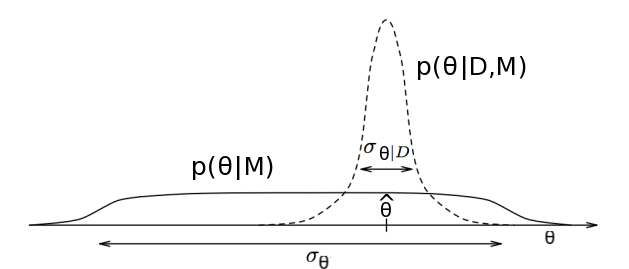
\includegraphics[scale=0.45]{hw3files/figs/posterior.png}
\caption{The posterior $p(\theta|\mathcal{D},\mathcal{M})$ and prior $p(\theta | \mathcal{M})$ over parameters $\theta$ under model $\mathcal{M}$.  
$\hat{\theta} = \text{argmax}_{\theta} 
p(\theta|\mathcal{D},\mathcal{M})$. }
\label{fig: posterior}
\end{figure}


\item (14 marks): The posterior $p(\bm{\theta} | \mathcal{M}, \mathcal{D}) \propto p(\mathcal{D} | \mathcal{M}, \bm{\theta}) p(\bm{\theta})$ will often be sharply peaked around its maximum value, as in Figure \ref{fig: posterior}.  The evidence in Eq.~\eqref{eqn: evidence} can thus be approximated by its height times its width $\sigma_{\theta | \mathcal{D}}$:
\begin{align}
\overbrace{p(\mathcal{D} | \mathcal{M})}^{\text{evidence}} \approx \overbrace{p(\mathcal{D} | \hat{\bm{\theta}}, \mathcal{M})}^{\text{data fit}} \overbrace{p(\hat{\bm{\theta}} | \mathcal{M}) \sigma_{\theta | \mathcal{D}}}^{\text{Occam factor}}
\end{align}
The evidence thus naturally compartmentalizes into data fit and Occam factor terms.  Suppose for simplicity that the prior is uniform on a large interval such that $p(\hat{\bm{\theta}} | \mathcal{M}) = 1/\sigma_{\theta}$.  The Occam's 
factor then becomes $\frac{\sigma_{\theta|\mathcal{D}}}{\sigma_{\theta}}$. 
\begin{enumerate}[label=(\alph*)]
\item (2 marks): Provide an interpretation of the Occam's factor $\frac{\sigma_{\theta|\mathcal{D}}}{\sigma_{\theta}}$, wrt Figure \ref{fig: occam}.
\item (4 marks): Show that if we use Laplace's method to approximate the posterior $p(\bm{\theta} | \mathcal{M}, \mathcal{D})$ 
as a Gaussian, then the Occam's factor becomes 
$p(\hat{\bm{\theta}} | \mathcal{M}) \text{det}(A)^{-1/2}$ where $A = -\nabla \nabla \log p(\bm{\theta} | \mathcal{D},\mathcal{M})$.  Use this expression to interpret each of the terms in the log marginal likelihood you derived for question 1(b).
\item (6 marks): Derive an approximation for the log evidence $\log p(D | \mathcal{M})$ assuming a broad Gaussian prior distribution and iid observations, strictly in terms of the number of datapoints $N$, the number of parameters $m$ (dimensionality of $\bm{\theta}$), and 
$\log p(D | \hat{\bm{\theta}})$.  Show all of your work.
\item (2 marks): Relate the Hessian $A$ to the covariance matrix of a Gaussian prior over parameters.
\end{enumerate}

\item (33 marks): Load the datasets $\mathcal{D}_1$ and $\mathcal{D}_2$ respectively from \texttt{occam1.mat} and \texttt{occam2.mat} in the assignment files \texttt{a3files.zip}.  Suppose we are considering three models to explain the data:
\begin{enumerate}[label=(\roman*)]
\item $\mathcal{M}_1$: The Bayesian basis regression model of Eq.(2)-(4), but with 
\begin{equation}
\bm{\phi}(x,\bm{z}) = \bm{\phi}(x) = (1,x,x^2,x^3,x^4,x^5)^{\top}
\end{equation}
\item $\mathcal{M}_2$: The Bayesian basis regression model of Eq.(2)-(4), but with 
\begin{equation}
\bm{\phi}(x,\bm{z}) =  \left( \exp[-\frac{(x-1)^2}{z_1^2}], \exp[-\frac{(x-5)^2}{z_2^2}] \right)^{\top}, \quad \bm{z} = (z_1,z_2)^{\top}
\end{equation}
\item $\mathcal{M}_3$: The Bayesian basis regression model of Eq.(2)-(4), but with 
\begin{equation}
\bm{\phi}(x,\bm{z}) =  \bm{\phi}(x) = (x,\cos(2x))^{\top}
\end{equation}
\end{enumerate}
Parts of this question involve coding.  Please hand in the Matlab, Octave, or Python code you used to solve this question, along with the plots of results generated by the code used to answer the questions.  This code should be succinct and include comments.  Your code should not exceed 5 pages in length.   Answer all questions for both $\mathcal{D}_1$ and $\mathcal{D}_2$ unless the question explicitly states otherwise.

\vspace{2mm}
\begin{enumerate}
\item (20 marks): Using your work from question 1, write code to plot a histogram of the evidence for each of these three models, conditioned on the maximum marginal likelihood values of all the hyperparameters $\bm{z}$, $\alpha^2$, and $\sigma^2$. To find these values, jointly optimize the log marginal likelihood with respect to these hyperparameters using a quasi-Newton method or non-linear conjugate gradients.  Based on the histogram, which hypotheses do you believe generated the data?  \\ 
\textbf{Hint 1}: If you compute the Cholesky decomposition of $A = R^{\top} R$, where $R$ is an upper right triangular matrix, then 
$A^{-1}\bm{b}$ = $R^{-1}(R^{-1})^{\top} \bm{b}$.  You can use this decomposition in conjunction with the helper function \texttt{solve\_chol.m} for numerically stable solutions to linear systems involving $A$.  
Note also that $\log \det(A) = 2 \sum_i \log(R_{ii})$. \\
\textbf{Hint 2}: Use the function \texttt{checkgrad.m}, or compute a finite difference scheme, to numerically check the derivatives of the log marginal likelihood with respect to the model hyperparameters, as a means to debug and to check your answer for 1(c). \\
\textbf{Hint 3}: Some of the relevant matrices may be very poorly conditioned.  It is often useful to add a constant small amount of \emph{jitter} to the diagonal of these matrices, $A \to A + \epsilon I$, where $\epsilon$ is on the order of $10^{-6}$, before performing operations such as Cholesky decompositions. This procedure is advocated by Radford Neal in his 1996 PhD thesis, \emph{Bayesian Learning for Neural Networks}. \\
\textbf{Hint 4}: You may wish to constrain your hyperparameters to be positive, but perform an unconstrained optimization.  To do so, you can optimize over the log hyperparameters in an unconstrained space.  When computing derivatives of the log marginal likelihood with respect to the log parameters, you will find it helpful to use the chain rule.\\
\textbf{Hint 5}: I have included \texttt{minimize.m}, a robust implementation of non-linear conjugate gradients you can use to optimize the marginal likelihood with respect to hyperparameters.  You are, however, free to use another gradient based optimizer if you wish.

\item (8 marks): Explain why the evidence histogram might disagree with the maximum likelihood ranking of models (in general and with respect to $\mathcal{D}_1$ and $\mathcal{D}_2$).
\item (2 marks): Give the posterior mean and variance over the parameters of the model with highest evidence on $\mathcal{D}_2$.
\item (3 marks): What values of the \emph{hyperparameters} maximized the marginal likelihood? 
\item Optional (1 bonus mark): Plot the posterior over each set of model weights $\bm{w}$  (using extra coding space if required) for each dataset.

\end{enumerate}

\end{enumerate}

\vspace{10mm}
\textbf{Markov chain Monte Carlo} \\
(15 marks)

Follow Iain Murray's MCMC practical at \\
\url{http://homepages.inf.ed.ac.uk/imurray2/teaching/09mlss/handout.pdf}

Complete section 4, and answer the MCMC questions in section 5.

Hand in (1) your code for section 4, and (2) your answers to the 5 MCMC questions.  The code is worth 10 marks, and the questions are worth 1 mark each.  There are thus 15 marks for this part of the assignment.


\end{document}

